\section{Problem Definition and Algorithm}
\subsection{Task Definition}
In this paper, we address the problem of sentiment analysis of Twitter message. To be more precise, 
given a message, we want to classify whether the message is of positive or negative (binary decision), or neutral sentiment (ternary decision). For messages conveying both a positive and negative sentiment, whichever is the stronger sentiment should be chosen. For the following two example message, we are expected to return positive on the first one and negative on the second. 
\begin{mdframed}[
  leftmargin=\parindent,
  rightmargin=\parindent,
  skipabove=\topsep,
  skipbelow=\topsep
  ]
  If u haven't seen \#Rio2 yet-GO! You need to meet Gabi! Great singer. Cute. Absolutely hysterical! @KChenoweth \url{pic.twitter.com/kkVBUKjqE3}
\end{mdframed}

\begin{mdframed}[
  leftmargin=\parindent,
  rightmargin=\parindent,
  skipabove=\topsep,
  skipbelow=\topsep
  ]
 The rio 2 has one of the worst soundtracks evvvvaaa. I'm at Alamo @Drafthouse Cinema. @marissanicole11 \url{http://4sq.com/1kKF8qE} 
\end{mdframed}

This task is interesting because sentiment of Twitter message can be used as a barometer for public mood and opinion in diverse areas such as entertainment, politics and economics. For example, 
it is used to provide information on the temporal dynamic of sentiment in reaction to the debate video between Barack Obama and John McCain\cite{Diakopoulos:2010}. 
There is also a report on "Berkshire Hathaway Stock Rises When Anne Hathaway Makes Headlines"\footnote{\url{http://goo.gl/WlfY1c}/}, which indicates that sentiment toward public figure may have potential influence over stock market. 

However, twitter message presents greater challenges for sentiment analysis than more traditional text genres, such as newswire data.  Tweets are within 140 characters, often consists of a few short sentences or even a single sentence. 
The language used is very informal, with creative spelling and punctuation, misspellings, slang, new words, URLs, and genre-specific terminology and abbreviations, such as, RT for “re-tweet” and \#hashtags, which are a type of tagging for Twitter messages. \footnote{\url{http://www.cs.york.ac.uk/semeval-2013/task2/}}


\subsection{Algorithm Definition}
We experiment with two different types of models: The first is the traditional bag-of-word model, namely SVM here. The other is the recently proposed Recursive Neural Tensor Network which works pretty good on movie reviews. As different model has different requirement on pre-processing, we first introduce the models we use and then the pre-processing steps. 


\subsubsection{SVM}

\newpage

\subsubsection{RNTN}
In Recursive Neural Tensor Network, each word is represented as a $d-$dimensional vector. When an $n-$gram is given to the compositional models, it is parsed into a binary tree (as in Figure \ref{trigram}). We compute the parent vector in a bottom up fashion using a compositionally function $g$ and use node vectors as features for a classifier at that node. 
\begin{figure}[H]
\begin{center}
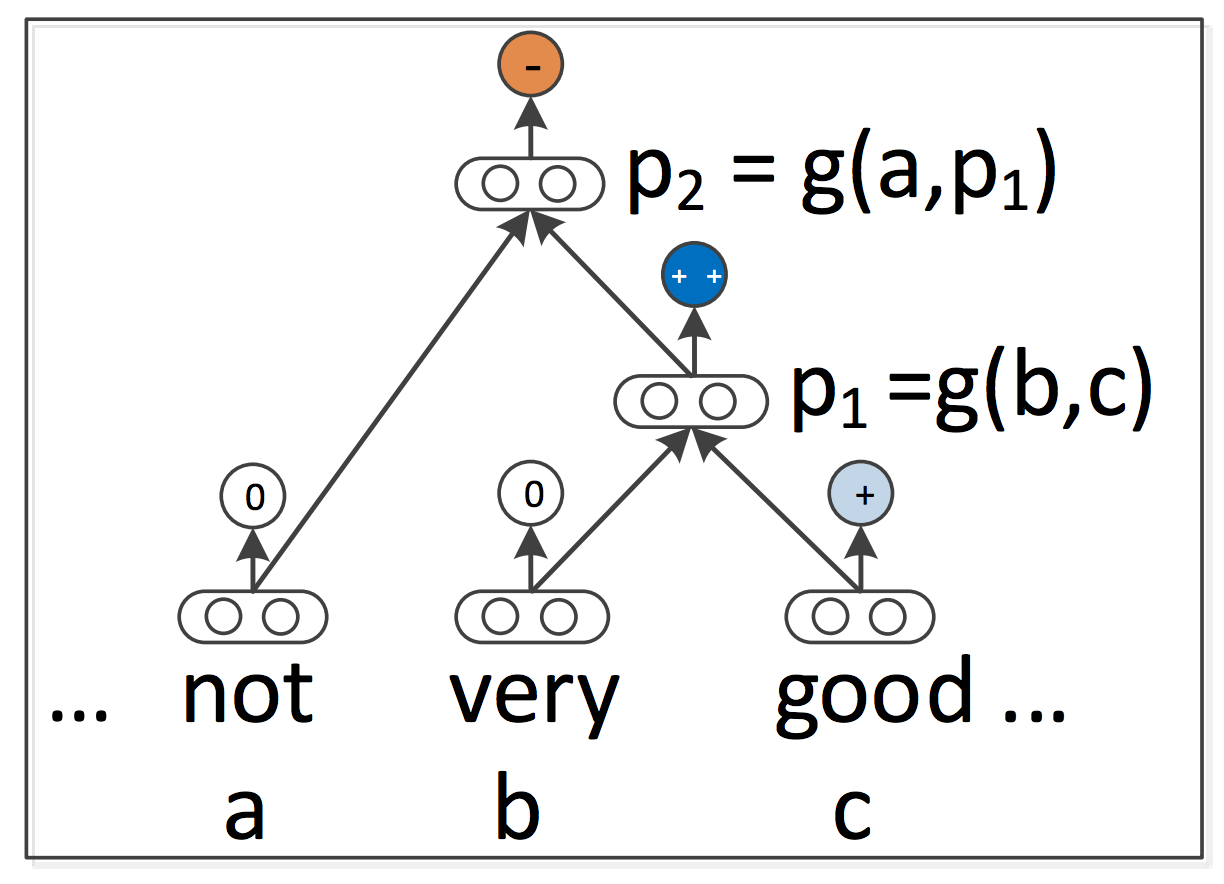
\includegraphics[width = 0.45\textwidth]{pic/trigram.png}
\caption{\label{trigram}Trigram Example (Socher et al., 2013) }
\end{center}
\end{figure}

RNTNs use the following equations to compute the parent vectors: 
\begin{equation*}
p_1 = f \left(  
\begin{bmatrix}
b \\ c
\end{bmatrix}^T
V^{[1:d]} 
\begin{bmatrix}
b \\ c
\end{bmatrix}
+ W
\begin{bmatrix}
b \\ c
\end{bmatrix}
 \right)
\end{equation*}
 
where $f = \textrm{tanh}$ is standard element-wise nonlinearity. $V^{[1:d] \in \mathbb{R}^{2d \times 2d \times d}}$ is the tensor that defines mulitiple bilinear forms. $W \in \mathbb{R}^{d \times 2d}$ is the main parameter to learn. 

The next parent vector $p_2$ in the tri-gram will be computed with the same weights:
\begin{equation*}
p_2 = f \left(  
\begin{bmatrix}
a \\ p_1
\end{bmatrix}^T
V^{[1:d]} 
\begin{bmatrix}
a \\ p_1
\end{bmatrix}
+ W
\begin{bmatrix}
a \\ p_1
\end{bmatrix}
 \right)
\end{equation*}

As we use the RNTN model as a black box in this project, so I skip the details on how to train the model. Interested reader could refer to the paper by Socher et al,. (2013). 


\subsubsection{Pre-processing}
\begin{itemize}
\item Twitter related features
\item Slangs
\item Emoticons
\item Spelling correction
\item Word Cluster
\end{itemize}


%Describe in reasonable detail the algorithm you are using to address this problem. A psuedocode description of the algorithm you are using is frequently useful. Trace through a concrete example, showing how your algorithm processes this example. The example should be complex enough to illustrate all of the important aspects of the problem but simple enough to be easily understood. If possible, an intuitively meaningful example is better than one with meaningless symbols. 

